\documentclass{article}
%preambulo
\usepackage[spanish]{babel}
\usepackage[utf8]{inputenc}
\usepackage{textcomp}
\usepackage{graphicx}
\graphicspath{ {images/} }
\usepackage{fancyhdr}
\usepackage[a4paper, margin=1in]{geometry}
\usepackage{listings}
\usepackage{color}
\usepackage[skins]{tcolorbox}
\usepackage{hyperref}
 
\definecolor{codegreen}{rgb}{0,0.6,0}
\definecolor{codegray}{rgb}{0.5,0.5,0.5}
\definecolor{codepurple}{rgb}{0.58,0,0.82}
\definecolor{backcolour}{rgb}{0.95,0.95,0.92}

\lstdefinestyle{mystyle}{
    backgroundcolor=\color{backcolour},   
    commentstyle=\color{codegreen},
    keywordstyle=\color{magenta},
    numberstyle=\tiny\color{codegray},
    stringstyle=\color{codepurple},
    basicstyle=\footnotesize,
    breakatwhitespace=false,         
    breaklines=true,                 
    captionpos=b,                    
    keepspaces=true,                 
    numbers=left,                    
    numbersep=5pt,                  
    showspaces=false,                
    showstringspaces=false,
    showtabs=false,                  
    tabsize=2,
    frame=single
}

\lstset{style=mystyle}


\title{Tutorial de Pilas-Engine}
\date{2018}
\pagestyle{fancy}
\fancyhf{}
\fancyhead[LE,RO]{Pilas-Engine}
\fancyhead[RE,LO]{Tutorial de Grillas y Animación}
\fancyfoot[LE,RO]{Pagina \thepage}
\fancyfoot[RE,LO]{2018}

\renewcommand{\headrulewidth}{2pt}
\renewcommand{\footrulewidth}{1pt}

%cuerpo documento
\begin{document}
\section{Grillas y Animación}
En el manual y en los ejemplos de \textbf{Pilas}, puedes ver cómo usar \textbf{grillas} para tener tus personajes animados de forma automática. Pero el tema es algo más complicado cuando quieres hacer que tengan comportamientos específicos que se coordinen con los diferentes fotogramas que forman parte del diseño. Vamos a ver cómo hacer esto, paso a paso.\par

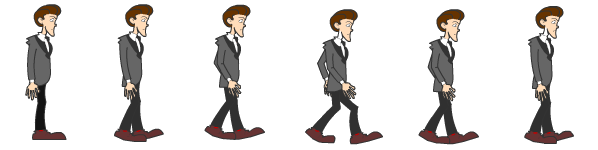
\includegraphics[width=\textwidth]{andando}

Partimos de un personaje (llamémoslo \textbf{chuck}) cuyo diseño descansa en la grilla superior; tenemos un primer fotograma o \textbf{cuadro} (en el lenguaje de Pilas) en posición de descanso, y otros 5 cuadros que muestran el movimiento del hombre andando. Éste es la planificación que vamos a seguir:\par

\begin{itemize}
\item \textbf{andando01.py}

Usaremos el primer cuadro y lo desplazaremos por la pantalla con los controles por
defecto que incorpora pilas (las flechas del cursor).\par
\item \textbf{andando02.py}

Aprenderemos a desplazar al actor con las teclas que queramos, usando el módulo
control.\par
\item \textbf{andando03.py}

Haremos que en el movimiento, el actor cambie de cuadro simulando el caminar. Lo
haremos manualmente y veremos sus limitaciones.\par
\item \textbf{andando04.py}

Aprenderemos de la experiencia de Pilas y de los actores que incorpora, usando el
módulo comportamientos y consiguiendo una animación más real y extensible.\par
\item \textbf{andando05.py}

Extenderemos el comportamiento del actor para que también salte, viendo las
ventajas que derivan del planteamiento del paso anterior.\par
\end{itemize}

\subsection{andando01.py}

\begin{lstlisting}[language=Python]
#! /usr/bin/env python
# -*- coding: utf-8 -*-
#-----------------------------------------------------------------------
# andando01.py
# Movimiento Automático
#-----------------------------------------------------------------------
import pilasengine

pilas=pilasengine.iniciar()

# Definimos la clase de nuestro actor
class Hombre(pilasengine.actores.Actor):
    """Un actor que se mueve con el teclado"""
    def iniciar(self):
        self.imagen=pilas.imagenes.cargar_grilla("andando.png",6)
        self.aprender("MoverseConElTeclado")
        
chuck=Hombre(pilas)

pilas.ejecutar()

\end{lstlisting}
Llegados a este punto, este paso tendría que estar claro (si no lo has hecho todavía,
tendrías que leer el tutorial de Mario \href{http://pilas-engine.com.ar/tutoriales/mario_renovado.pdf}{aqui}). Hemos definido la clase de actor \textbf{Hombre} y luego la hemos \textbf{instanciado}, creando un actor de ese tipo al que hemos llamado, \textbf{chuck}.\par
Dos matices nuevos. Primero, la imagen de chuck la cargamos usando el método \textbf{cargar\_grilla()}. Con éste método hemos de indicar el número de cuadros que forman la grilla (en nuestro caso, 6). Es muy importante el que tengamos en cuenta que Pilas divide entonces la imagen de referencia en un mosaico de piezas iguales para usarlas; nuestros cuadros deben ser todos del mismo tamaño.\par
Por otra parte, conseguir que un actor se mueva con los controles que proporciona Pilas por defecto es muy sencillo. Basta usar el método \textbf{aprender()} del actor y pasarle como argumento la habilidad \textbf{MoverseConElTeclado} como string. A partir de ese momento, nuestro chuck se moverá con las flechas del cursor (izquierda, derecha, arriba y abajo).\par
Prueba (da al código el nombre \textbf{andando01.py}) y ejecútalo. Y si quieres aprender más del movimiento por defecto con el teclado, usa \textbf{dir()}, \textbf{help()} o \textbf{pilas.ver()} en el intérprete.\\

\vspace{\baselineskip}
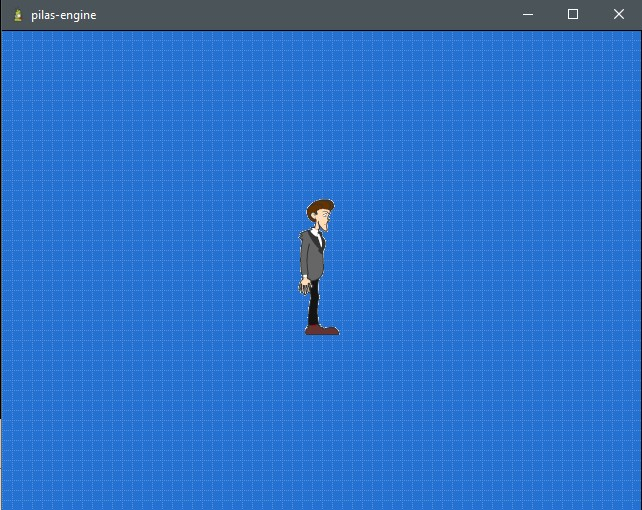
\includegraphics[width=\textwidth]{andando01}
\vspace{\baselineskip}

Hay otras habilidades que podrías usar con el actor. Por ejemplo, cuando lo mueves, es fácil que se salga de la pantalla. Puedes controlarlo a partir de las coordenadas y del tamaño de la ventana, pero hay una forma automática para ello, y es aprender la habilidad \textbf{SeMantieneEnPantalla}; una vez hecho esto, por mucho que lo intentes, chuck se mantendrá siempre dentro de los límites de la ventana. Para ver un listado completo de las habilidades puedes entrar \href{http://manual.pilas-engine.com.ar/habilidades/#listado-de-habilidades-existentes}{aqui}.\par
Y ¿qué sucede si queremos manejar a nuestro personaje con otras teclas diferentes? 
Avancemos al siguiente paso, en el que usaremos las teclas \textbf{a} y \textbf{s} para mover al actor hacia la izquierda y la derecha, respectivamente.\par
\vspace{\baselineskip}

\subsection{andando02.py}

\begin{lstlisting}[language=Python]
#! /usr/bin/env python
# -*- coding: utf-8 -*-
#-----------------------------------------------------------------------
# andando02.py
# Movimiento con controles propios
#-----------------------------------------------------------------------
import pilasengine

pilas=pilasengine.iniciar()

# Definimos las teclas que moverán al personaje
teclas = {pilas.simbolos.a:"izquierda", pilas.simbolos.s:"derecha"}

# Creamos un control personalizado con esas teclas
mandos=pilas.control.Control(teclas)

# Definimos la clase de nuestro actor
class Hombre(pilasengine.actores.Actor):
    """Un actor que se mueve con las teclas a y s"""
    def iniciar(self):
        self.imagen=pilas.imagenes.cargar_grilla("andando.png",6)
# Hacemos que el actor se mueva con nuestro control personalizado
        self.aprender("MoverseConElTeclado",control=mandos)
        
chuck=Hombre(pilas)

pilas.ejecutar()

\end{lstlisting}

\vspace{\baselineskip}
Lo primero que notarás es la siguiente línea:
\begin{lstlisting}[language=Python]
teclas= {pilas.simbolos.a:"izquierda", pilas.simbolos.s:"derecha"}
\end{lstlisting}
\vspace{\baselineskip}

La variable \textbf{teclas} es un \textbf{diccionario}. Ésta es la manera que usa Pilas para definir controles. Los diccionarios están formados por parejas; la llamada \textbf{clave} y su \textbf{valor} correspondiente. En el caso de los controles de Pilas, \textbf{en la clave indicaremos la tecla} que deseemos mientras que \textbf{en el valor pondremos la dirección} del movimiento. Usa \textbf{help (pilas.simbolos)}, por ejemplo, para ver las teclas predefinidas. En nuestro caso, vamos a usar la tecla \textbf{a} para el movimiento hacia la izquierda y la tecla \textbf{s} para la derecha.\par
Lo siguiente es crean un objeto que controle esas teclas y que nos permita utilizarlo para manejar a chuck. Eso lo logramos con la siguiente línea:
\begin{lstlisting}[language=Python]
mandos = pilas.control.Control(teclas)
\end{lstlisting}
\vspace{\baselineskip}

Los objetos de la clase \textbf{pilas.control.Control} se encargan, precisamente, de la tarea que deseamos. Al constructor de la clase, como vemos, sólo tenemos que pasarle el \textbf{diccionario} que hemos definido con las \textbf{teclas} que vamos a usar.\par
Una vez que tenemos el \textbf{nuevo control} definido, al que hemos llamado \textbf{mandos}, podemos usarlo con el actor que queramos. ¿Recuerdas que en el paso anterior, para usar las teclas que trae por defecto Pilas, hemos usando en la definición de chuck lo siguiente?
\begin{lstlisting}[language=Python]
self.aprender("MoverseConElTeclado")
\end{lstlisting}
\vspace{\baselineskip}

Bien, pues esa línea la hemos de cambiar por esta otra:
\begin{lstlisting}[language=Python]
self.aprender("MoverseConElTeclado",control=mandos)
\end{lstlisting}

\vspace{\baselineskip}
¿Ves qué simple? Simplemente hemos de incluir un argumento más, llamado \textbf{control}, con  el objeto que contiene el control de teclado que hemos definido (nuestro \textbf{mandos}).\par
¡Pruébalo! Si ejecutas el código con el nombre \textbf{andando02.py}, verás que ahora puedes mover a chuck con las teclas \textbf{a} y \textbf{s} y ya no se puede mover en dirección vertical.\par
La verdad es que queda un poco soso e irreal. Una imagen fija desplazándose por la 
pantalla... ¡Usemos la grilla y que cambie el aspecto de chuck con el movimiento!
Para eso, hemos de saltar al siguiente paso.\par

\subsection{andando03.py}
\begin{lstlisting}[language=Python]
#! /usr/bin/env python
# -*- coding: utf-8 -*-
#-----------------------------------------------------------------------
# andando03.py
# Movimiento simple manual con uso de grilla
#-----------------------------------------------------------------------
import pilasengine

pilas=pilasengine.iniciar()

# Definimos las teclas que moveran al personaje
teclas = {pilas.simbolos.a:"izquierda", pilas.simbolos.s:"derecha"}

# Creamos un control personalizado con esas teclas
mandos=pilas.control.Control(teclas)

# Definimos la clase de nuestro actor
class Hombre(pilasengine.actores.Actor):
    """Un actor que se mueve con las teclas a y s y con animacion"""
    def iniciar(self):
        self.imagen=pilas.imagenes.cargar_grilla("andando.png",6)
        self.cuadro=0
        # Hacemos que el actor se mueva con nuestro control personalizado
        self.aprender("MoverseConElTeclado",control=mandos)
    
    def actualizar(self):
        # Miramos si se han pulsado las teclas adecudas para cambiar, en
        # su caso, la imagen de la grilla y hacia donde mira
        if mandos.izquierda:
            if not self.espejado:
                self.espejado = True
            self.cuadro+=1
        elif mandos.derecha:
            if self.espejado:
                self.espejado = False
            self.cuadro+=1
        else:
            self.cuadro=0
        if self.cuadro>5:
            self.cuadro=1
            
        self.imagen.definir_cuadro(self.cuadro)
                
            
        
chuck=Hombre(pilas)

pilas.ejecutar()

\end{lstlisting}
\vspace{\baselineskip}

La idea es que, en cada paso, el cuadro de animación de la grilla de chuck, cambie.\par
¡Importante! Recuerda que las listas y demás \textbf{elementos iterables}, en \textbf{Python}, se numeran empezando por el \textbf{0}, no por el 1. Así que los 6 cuadros de nuestra grilla están numerados de la siguiente forma:\par

\vspace{\baselineskip}
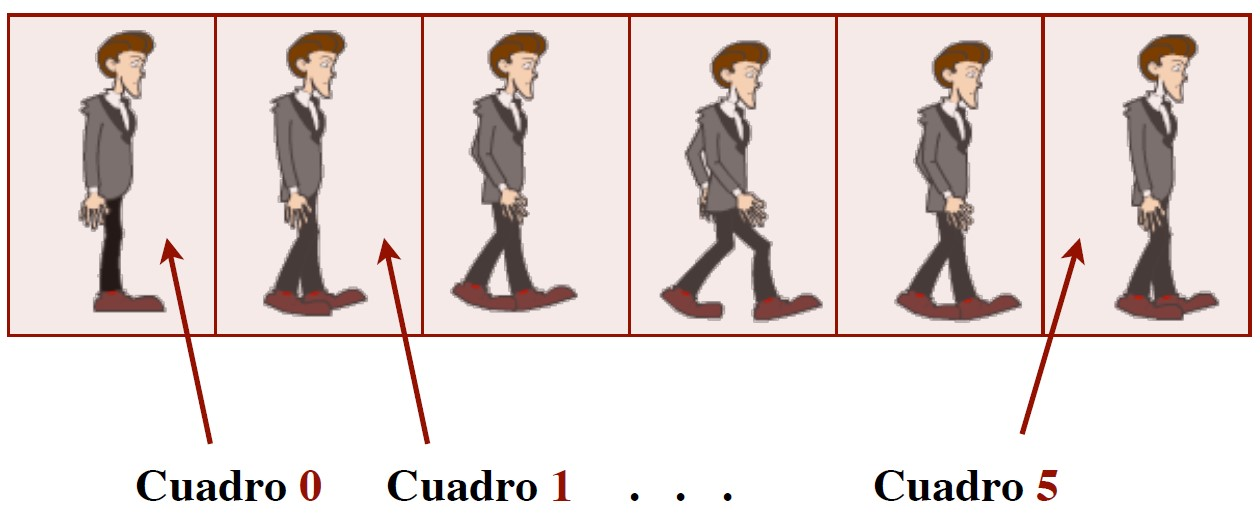
\includegraphics[width=\textwidth]{grilla_numerada}

Bien. Tenemos que usar una variable que controle el cuadro que está en activo en cada momento, así que la hemos definido como \textbf{cuadro} (es decir, \textbf{self.cuadro} para que quede almacenada con el Actor) e inicialmente le damos el valor \textbf{0}, ya que la posición de partida de chuck es la que está parado.\par
Y ¿cómo cambiamos de cuadro? ¿Recuerdas que, en cada fotograma de la animación, Pilas llama al método \textbf{actualizar()} de cada Actor? ¡Éste es el lugar! Así que añadimos su definición a la clase de actor \textbf{Hombre}, para darle un comportamiento personalizado.\par
Lo primero que hemos de hacer, dentro del método \textbf{actualizar()}, es ver si se está pulsando la tecla que mueve a chuck hacia la izquierda o la que lo mueve hacia la derecha o ninguna de las dos. Esto es lo que conseguimos con
\begin{lstlisting}[language=Python]
if mandos.izquierda:
        ...
elif mandos.derecha:
        ...
else:
\end{lstlisting}
\vspace{\baselineskip}

Después de definir \textbf{mandos} (como un objeto de tipo \textbf{pilas.control.Control}), es muy fácil determinar si se ha pulsado la tecla que queremos. Si, por ejemplo, se ha pulsado la tecla que hemos definido como movimiento hacia la izquierda, \textbf{mandos.izquierda} es \textcolor{codepurple}{\textbf{True}} (y \textcolor{codepurple}{\textbf{False}} en caso contrario). Así que, en el esqueleto anterior, miramos si chuck ha de moverse hacia la izquierda (para hacer lo propio), si no, miramos si hay que moverlo hacia la derecha y, finalmente, en caso contrario (y a través del \textcolor{codepurple}{\textbf{else}}) hacemos lo correspondiente a cuando chuck tenga que estar parado.\par
Es evidente que, en cada uno se esos casos, hemos de indicar qué cuadro ha de ser el que empleemos en el dibujado de nuestro personaje. Empezando por el último, lo más sencillo, como el cuadro correspondiente al estado de parado es el número \textbf{0}, escribimos

\begin{lstlisting}[language=Python]
self.cuadro = 0
\end{lstlisting}
\vspace{\baselineskip}

Por lo demás, cuando salgamos del \textbf{bloque} \textcolor{codepurple}{\textbf{if}} con el cuadro que debemos usar adjudicado,  ¿cómo se lo indicamos a Pilas?. Las \textbf{grillas} tienen un método definido para eso. Se trata del método \textbf{definir\_cuadro()}, al que le debemos pasar, como es lógico, el cuadro deseado. Eso es lo que hacemos con\par

\begin{lstlisting}[language=Python]
self.imagen.definir_cuadro(self.cuadro)
\end{lstlisting}
\vspace{\baselineskip}

ya que el atributo \textbf{self.imagen} del actor contiene la grilla de chuck que hemos cargado en memoria en su \textbf{iniciar(self)}.\par
Lo único que nos falta por comprender es lo que hay que hacer cuando se ha pulsado la tecla \textbf{a} (es decir, cuando \textbf{mandos.izquierda} es \textcolor{codepurple}{\textbf{True}}) o la tecla \textbf{s}. Como ambas funcionan de forma parecida, vamos a fijarnos en el primer caso. Ésta es la parte del código que hemos de analizar:\par

\begin{lstlisting}[language=Python]
if mandos.izquierda:
    if not self.espejado:
        self.espejado = True
    self.cuadro += 1
\end{lstlisting}
\vspace{\baselineskip}

Fijando ideas, hay dos cosas que hemos de hacer (recordando que, como chuck ha 
aprendido la habilidad \textbf{MoverseConElTeclado}, ya se desplaza por la pantalla al pulsar las teclas, así que no hemos de preocuparnos de cambiar su coordenada \textbf{x}):\par

\begin{itemize}
\item Cambiar el cuadro de la animación.
\item Asegurarse de que chuck mira en la dirección en la que está andando.
\end{itemize}
Lo primero es fácil, basta con aumentar en \textbf{1} la variable que controla en qué cuadro de la animación estamos.\par
Lo segundo cuesta algo más, pero tampoco es complicado. Si te fijas en la grilla de nuestro personaje, verás que en todos los casos está mirando hacia la derecha. Así que la imagen, \textbf{en su estado normal}  (es decir, cuando el valor del atributo \textbf{self.espejado} del actor tiene su valor por defecto, \textcolor{codepurple}{\textbf{False}}), \textbf{mira hacia la derecha}. ¿Qué debemos hacer entonces? Lo que le debemos decir a Pilas es algo como lo siguiente: “Hey, si se ha de mover a la izquierda y la imagen está mirando a la derecha, cámbiala”. Si ya está mirando hacia la izquierda, no hace falta, ¿no?...\par
Manos a la obra. Si chuck está mirando hacia la derecha, \textbf{self.espejado} es \textcolor{codepurple}{\textbf{False}}, así que \textcolor{codepurple}{\textbf{not}} \textbf{self.espejado} será \textcolor{codepurple}{\textbf{True}}. Y es en este caso cuando hay que hacer que mire hacia la izquierda, así que hay que decirle que cambie \textbf{self.espejado} a \textcolor{codepurple}{\textbf{True}}. Esto es lo que hacen las dos líneas en el caso de que se halla pulsado la tecla \textbf{a} (\textbf{mandos.izquierda} es \textcolor{codepurple}{\textbf{True}})\par

\begin{lstlisting}[language=Python]
if not self.espejado:
    self.espejado = True
\end{lstlisting}
\vspace{\baselineskip}

En el caso de que se halla pulsado la tecla \textbf{s} y debamos movernos hacia la derecha, ocurre algo parecido pero en sentido inverso, pues hay que asegurarse que \textbf{self.espejado} es en ese caso \textcolor{codepurple}{\textbf{False}}.\par
Una ultima cosa. ¡No te olvides que tenemos solo 6 cuadros en la grilla! La parte en la que nuestro personaje anda, empieza en el cuadro número \textbf{1} y termina en el cuadro número \textbf{5}. Así que cuando sumamos \textbf{1} a la variable \textbf{self.cuadro}, hemos de asegurarnos de que no nos pasamos de dichos números. Es por eso por lo que hemos añadido\par

\begin{lstlisting}[language=Python]
if self.cuadro > 5:
    self.cuadro = 1
\end{lstlisting}
\vspace{\baselineskip}
justo antes de asignar el cuadro que hay que dibujar con el método \textbf{definir\_cuadro()}.\par
¡De acuerdo, el movimiento se demuestra andando! Guarda todo el código anterior con el nombre \textbf{andando03.py} y ejecútalo. ¿Puedes ver cómo se mueve chuck?\par

\vspace{\baselineskip}
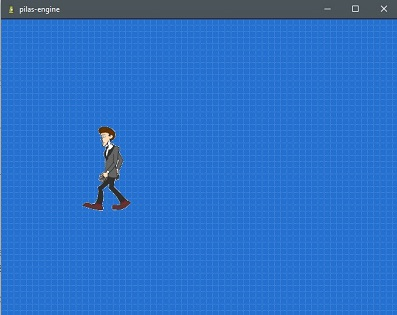
\includegraphics{andando02}

\subsection{andando04.py}

Después de mirar el resultado del paso anterior, sólo podemos llegar a una conclusión:
¡chuck tiene el Baile de San Vito!
Esos movimientos tan convulsivos en los andares de nuestro personaje son consecuencia
de la manera grosera con la que hemos abordado los cambios de cuadro de la animación.
Para empezar, en cada llamada de Pilas al método actualizar() del actor se cambia de
cuadro. ¿A qué velocidad, en fotogramas por segundo, ocurre esto? Y ¿cuántos píxeles
avanza en cada paso? En una animación correcta, deberíamos controlar estos factores.
Hay diferentes metodologías para abordar esta cuestión. Pero estamos aquí para aprender
de Pilas y ésta es una buena excusa para ello...\par

\vspace{\baselineskip}

\begin{tcolorbox}[skin=widget,
boxrule=1mm,
coltitle=black,
colframe=blue!45!white,
colback=white,
width=(.9\linewidth),before=\hfill,after=\hfill,
adjusted title={Más Código Fuente de Pilas}]

Un paso más avanzado en la compresión del funcionamiento de Pilas lo puedes obtener al examinar su código fuente.\par
Hasta ahora hemos usado, para hacernos una idea, las funciones dir(), help() y pilas.ver() en el intérprete de Pilas. Pero puedes aprender más, todavía, husmeando entre las líneas de su \textbf{código fuente completo}.\par
Según cual sea la instalación de Pilas que tengas, es posible que no tengas acceso fácil a los archivos .py que lo constituyen (y a las imágenes y demás recursos multimedia). Deberían residir en una \textbf{carpeta pilas} en tu disco duro.\par
En cualquier caso, siempre podrás descargarlo desde la web de Pilas\par

\vspace{\baselineskip}
\begin{center}
\href{http://www.pilas-engine.com.ar}{http://www.pilas-engine.com.ar}
\end{center}
\vspace{\baselineskip}

y, tras descomprimirlo, estudiarlo.\par

En lo que sigue, vamos a referirnos al código del actor \textbf{Pingu}, que puedes encontrar en la \textbf{carpeta actores}, dentro de la \textbf{carpeta pilas}, con el nombre \textbf{pingu.py}. Si lo abres con tu editor (por ejemplo, Ninja-IDE), verás que, a parte del código de la clase \textbf{Pingu}, a la que tienes acceso con pilas.ver(), tienes el código de otras clases que complementan su definición:\par
  
\begin{lstlisting}[language=Python]
class Esperando(Comportamiento):
    "Un actor en posicion normal o esperando a que ..."
    ....
 class Caminando(Comportamiento):
    ....
 class Saltando(Comportamiento):
    ....
\end{lstlisting}

\end{tcolorbox}
\vspace{\baselineskip}

Pilas incorpora una serie de actores predefinidos con comportamientos que cubren la mayor parte de las necesidades típicas de los videojuegos. ¿Por qué no aprender de ello? En concreto, tenemos uno de ellos, \textbf{Pingu}, que posee una grilla y que avanza de la misma manera que lo hace chuck. Pero, claro, mucho mejor. Ésta es la grilla de Pingu (la puedes encontrar en la \textbf{carpeta data} dentro de la \textbf{carpeta pilas}, con el nombre \textbf{pingu.png}):\par


\vspace{\baselineskip}
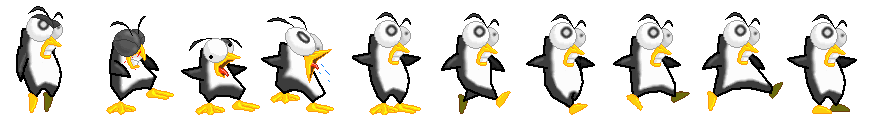
\includegraphics[width=\textwidth]{pingu}
\vspace{\baselineskip}

Si abres el intérprete de Pilas y juegas con él (crea una instancia de este tipo de actor escribiendo \textbf{pilas.actores.Pingu()}), verás que se desplaza de una forma similar a lo que deseamos (con la diferencia de que no usa el espejado y salta). De los cuadros que forman su grilla, la posición ‘en reposo’ es la número \textbf{4} y el caminar se forma con los cuadros del \textbf{5} al \textbf{9}.\par
¿Aprendemos de su código? Su método \textbf{iniciar()} es el siguiente:\par

\begin{lstlisting}[language=Python]
 def iniciar(self, x, y):
        self.x = x
        self.y = y
        self.imagen = self.pilas.imagenes.cargar_grilla("pingu.png", 10)
        self.definir_cuadro(4)
        self.hacer_inmediatamente(Esperando)
        self.radio_de_colision = 30
        self.centro = ("centro", "abajo")
        self.velocidad = 4
\end{lstlisting}
\vspace{\baselineskip}  

No hace falta que lo comprendamos todo al cien por cien. Fíjate sólo en un par de cosas.
Para empezar, que la grilla consta, como sabemos, de \textbf{10} cuadros y que se adjudica por
defecto el cuadro \textbf{4} (como también sabemos que debe ser). La forma de hacer esto último
tiene su matiz, pues en lugar de acceder directamente al método \textbf{definir\_cuadro()} de la
grilla, se usa un método definido en el propio \textbf{Pingu}, más adelante, para que sea más
accesible desde otros puntos del programa: en lugar de referirse a él como
\textbf{imagen.defini\_cuadro()} podemos poner, directamente, \textbf{definir\_cuadro()}. Es una
cuestión de estilo.\par
Esto es lo fundamental: \textbf{se usa el concepto de Comportamiento
para definir qué debe hacer Pingu}. ¿Qué comportamiento le adjudicamos? Éste:

\begin{lstlisting}[language=Python]
 self.hacer_inmediatamente(Esperando)
\end{lstlisting}
\vspace{\baselineskip}

¿Entiendes el proceso? Como puedes comprobar usando \textbf{help()}, el método \textbf{hacer\_inmediatamente()} de un
actor define el comportamiento de manera inmediata. Así que el quid de la cuestión está en
cómo se define el comportamiento que hemos denominado \textbf{Esperando}. Ya hemos visto,
en el recuadro de más arriba, que su definición está en el mismo archivo \textbf{pingu.py}.
De la misma manera que un actor genérico reside en el módulo \textbf{pilas.actores} y usamos
\textbf{pilas.actores.Actor} como el padre del cual derivar los demás, los comportamientos
residen en el módulo \textbf{pilas.comportamientos} y el progenitor de todos ellos es pilas.comportamientos.Comportamiento. Eso sí, por abreviar el código, en el
archivo pingu.py se importan las librerías de manera que podamos usar directamente sus
nombres... Éste es el código de la clase de comportamiento Esperando de Pingu:

\begin{lstlisting}[language=Python]
 class Esperando(Comportamiento):
    """Un actor en posición normal o esperando a que el usuario
    pulse alguna tecla.
    """

    def iniciar(self, receptor):
        self.receptor = receptor
        self.receptor.definir_cuadro(4)
        self.control = receptor.pilas.escena_actual().control

    def actualizar(self):
        if self.control.izquierda:
            self.receptor.hacer_inmediatamente(Caminando)
        elif self.control.derecha:
            self.receptor.hacer_inmediatamente(Caminando)

        if self.control.arriba:
            self.receptor.hacer_inmediatamente(Saltando)
\end{lstlisting}
\vspace{\baselineskip}

Pilas llama, tras crear un comportamiento, a su método \textbf{iniciar()} pasándole como argumento (\textbf{receptor}) el objeto al que se le va a asociar. En nuestro caso, \textbf{receptor} se refiere a \textbf{Pingu} y podemos ver cómo se insiste en indicar que el cuadro por defecto es el \textbf{4}.\par
¿Qué encontramos en el familiar método \textbf{actualizar()} que, recordemos, se llama en cada fotograma de la animación de Pilas? Debería ya ser fácil de entender: se mira el control del teclado y, si se ha pulsado una tecla de movimiento, se procede al comportamiento correspondiente. Nos interesa el comportamiento \textbf{Caminando}. Su definición está, de nuevo, en el mismo archivo \textbf{pingu.py} más adelante:

\clearpage
\begin{lstlisting}[language=Python]
class Caminando(Comportamiento):
    """Representa al personaje caminando por el escenario."""

    def iniciar(self, receptor):
        self.receptor = receptor
        self.cuadros = [5, 5, 6, 6, 7, 7, 8, 8, 9, 9]
        self.paso = 0
        self.control = receptor.pilas.escena_actual().control

    def actualizar(self):
        self.avanzar_animacion()
    ...
\end{lstlisting}
\vspace{\baselineskip}

Sólo hemos puesto las primeras líneas del código del comportamiento \textbf{Caminando}, pues ya entraremos en detalles en seguida, cuando pasemos a nuestro chuck. Basta que veamos que se indica la lista de cuadros que formarán parte de la animación del comportamiento (¿recuerdas la grilla de \textbf{Pingu}?). Observa que aparecen por duplicado; eso hará que se muestre más lenta la transición al tener que pasar por el doble de cuadros.\par
\textbf{En resumen de todo lo que hemos visto}: para conseguir que nuestro personaje responda de un modo específico, \textbf{tenemos que definir comportamientos y aplicárselos con el método hacer\_inmediatamente()}.\par
Ya estamos en condiciones de atacar nuestra mejora para chuck. ¡Aquí va!\par

\begin{lstlisting}[language=Python]
#! /usr/bin/env python
# -*- coding: utf-8 -*-
#-----------------------------------------------------------------------
# andando04.py
# Movimiento animado personalizado usando grilla
#-----------------------------------------------------------------------
import pilasengine

pilas=pilasengine.iniciar()

VELOCIDAD=4

# Definimos las teclas que moveran al personaje
teclas = {pilas.simbolos.a:"izquierda", pilas.simbolos.s:"derecha"}

# Creamos un control personalizado con esas teclas
mandos=pilas.control.Control(teclas)

# Definimos la clase de nuestro actor
class Hombre(pilasengine.actores.Actor):
    """Un actor que se mueve con las teclas a y s y con animación"""
    def iniciar(self):
        self.imagen=pilas.imagenes.cargar_grilla("andando.png",6)
        self.definir_cuadro(0)
        # Hacemos que el actor se mueva con nuestro control personalizado
        self.hacer_inmediatamente(Esperando)
    
    def definir_cuadro(self, indice):
        self.imagen.definir_cuadro(indice)
    
class Esperando(pilasengine.comportamientos.Comportamiento):
    """Actor en posicion normal o esperando a que el usuario pulse alguna tecla"""
    def iniciar(self, receptor):
        self.receptor= receptor
        self.receptor.definir_cuadro(0)

    def actualizar(self):
        if mandos.izquierda:
            self.receptor.hacer_inmediatamente(Caminando)
        elif mandos.derecha:
            self.receptor.hacer_inmediatamente(Caminando)
        
class Caminando(pilasengine.comportamientos.Comportamiento):
    """Actor caminando"""
    def iniciar(self, receptor):
        self.receptor = receptor
        self.cuadros = [1, 1, 1, 2, 2, 2, 3, 3, 3, 4, 4, 5, 5, 5, 5]
        self.paso = 0

    def actualizar(self):
        self.avanzar_animacion()
        
        if mandos.izquierda:
            if not self.receptor.espejado:
                self.receptor.espejado = True
            self.receptor.x-=VELOCIDAD
        elif mandos.derecha:
            if self.receptor.espejado:
                self.receptor.espejado = False
            self.receptor.x+=VELOCIDAD
        else:
           self.receptor.hacer_inmediatamente(Esperando)
    
    def avanzar_animacion(self):
        self.paso +=1
        if self.paso >= len(self.cuadros):
            self.paso=0
        
        self.receptor.definir_cuadro(self.cuadros[self.paso])
                
            
        
chuck=Hombre(pilas)

pilas.ejecutar()
\end{lstlisting}
\vspace{\baselineskip}

En primer lugar, definimos la constante \textbf{VELOCIDAD} que usaremos más adelante para controlar cuántos píxeles avanzará chuck en cada paso. Recuerda el convenio que usamos para los nombres; poner las constantes en mayúsculas nos sirve para identificarlas rápidamente.\par
Pasando a la definición de la clase del actor, nos encontramos con la función\par

\begin{lstlisting}[language=Python]
def definir_cuadro(self, indice):
    self.imagen.definir_cuadro(indice)
\end{lstlisting}
\vspace{\baselineskip}

que, como hemos dicho antes, nos permite cambiar el cuadro de la animación de chuck sin necesidad de acceder directamente a la grilla. Esto es precisamente lo que hacemos en el método \textbf{iniciar()}, indicando que el cuadro 0 es el cuadro en reposo por defecto. Y, a continuación, es donde establecemos también el comportamiento inicial del personaje; nuestro conocido \textbf{Esperando}.\par
Pasemos al quid de la cuestión; la implementación de los comportamientos de chuck. Tenemos dos; chuck parado (que se corresponde con \textbf{Esperando}) y chuck caminando (que se corresponderá con \textbf{Caminando}). Hay que tener en cuenta que en cualquier momento se puede pasar de un comportamiento al otro (basta con que el jugador pulse o deje de pulsar la tecla apropiada), así que debemos implementarlo en el código. Éste es el de \textbf{Esperando}:\par

\begin{lstlisting}[language=Python]
class Esperando(pilasengine.comportamientos.Comportamiento):
    """Actor en posicion normal o esperando a que el usuario pulse alguna tecla"""
    def iniciar(self, receptor):
        self.receptor= receptor
        self.receptor.definir_cuadro(0)

    def actualizar(self):
        if mandos.izquierda:
            self.receptor.hacer_inmediatamente(Caminando)
        elif mandos.derecha:
            self.receptor.hacer_inmediatamente(Caminando)
\end{lstlisting}
\vspace{\baselineskip}

¿Te resulta familiar la estructura? ¿La comprendes? En el método \textbf{iniciar()} del
comportamiento recogemos la referencia al personaje al que se lo vamos a aplicar en la
variable \textbf{receptor} y ponemos su cuadro a \textbf{0}, como ya sabemos. Nada más. Y en el método
\textbf{actualizar()} nos aseguramos de que si se pulsa la tecla \textbf{a} o la tecla \textbf{s}, se cambie el
comportamiento a \textbf{Caminando}.\par
¡No es tan difícil! ¿Qué hay del código de Caminando? Veamos:

\begin{lstlisting}[language=Python]
class Caminando(pilasengine.comportamientos.Comportamiento):
    """Actor caminando"""
    def iniciar(self, receptor):
        self.receptor = receptor
        self.cuadros = [1, 1, 1, 2, 2, 2, 3, 3, 3, 4, 4, 5, 5, 5, 5]
        self.paso = 0

    def actualizar(self):
        self.avanzar_animacion()
        
        if mandos.izquierda:
            if not self.receptor.espejado:
                self.receptor.espejado = True
            self.receptor.x-=VELOCIDAD
        elif mandos.derecha:
            if self.receptor.espejado:
                self.receptor.espejado = False
            self.receptor.x+=VELOCIDAD
        else:
           self.receptor.hacer_inmediatamente(Esperando)
    
    def avanzar_animacion(self):
        self.paso +=1
        if self.paso >= len(self.cuadros):
            self.paso=0
        
        self.receptor.definir_cuadro(self.cuadros[self.paso])
\end{lstlisting}
\vspace{\baselineskip}

Éste es un poco más largo, pero si lo desgranamos deberías comprenderlo bien.\par
Notarás que en el método \textbf{iniciar()} definimos dos variables; una con la lista de cuadros que forman la animación, \textbf{self.cuadros}, y otra que llevará la cuenta de cuál es el cuadro que está en activo en cada momento, \textbf{self.paso} (a \textbf{0} inicialmente, que indica el primer cuadro de la lista, es decir, el cuadro \textbf{1}). Si somos unos verdaderos artistas, tendremos mucho detalle en los diferentes fotogramas que forman la animación de un actor y parecerá un movimiento extremadamente real. Como no es el caso y hemos usado un sprite que hemos descargado directamente de internet, hemos triplicado la referencia a cada cuadro para que ésta se muestre más lenta y progresiva.\par
El método que se encarga de avanzar los cuadros en la animación, no podía llamarse de otro modo, es \textbf{avanzar\_animacion()}. Fíjate que lo que hace es muy transparente: Añade \textbf{1} a la variable \textbf{paso}, si ésta es mayor que el número de cuadros que hay en la lista (lo que se averigua con la función \textbf{len()}) se resetea a \textbf{0} (es decir, el primer cuadro de la lista) y se invica al método \textbf{definir\_cuadro()} del personaje indicando a cuál hay que cambiar.\par
Bien. Esto nos deja en el método \textbf{actualizar()} que es donde debemos mirar qué tecla se está pulsando para hacer una cosa u otra. Observa su código...\par
Lo primero, no en vano estamos caminando, es avanzar un cuadro en la animación del movimiento usando el método que acabamos de ver, \textbf{avanzar\_animacion()}. Lo siguiente es mirar el control del teclado que hemos definido, \textbf{mandos}, y ver si pulsamos la tecla \textbf{a} o la tecla \textbf{s}. En caso contrario, fíjate en el \textcolor{codepurple}{\textbf{else}}, se cambia el comportamiento a \textbf{Esperando}. ¡Claro!\par
Supongamos, por ejemplo, que se ha pulsado la tecla \textbf{a} para desplazar a chuck hacia la izquierda. Aquí hacemos algo similar a lo que hicimos en el paso anterior con el espejado del actor, ¿recuerdas? Pero además, hemos de avanzar a chuck para que no se quede en el sitio, de ahí que restemos la constante \textbf{VELOCIDAD} a su coordenada x. Y en el caso de que se pulse la tecla \textbf{s}, hemos de hacer lo mismo pero aumentando su coordenada x.\par
Pruébalo tu mismo. Guarda todo el código con el nombre \textbf{andando04.py} y ejecútalo. Notarás que la animación es mucho más suave. Y sólo cambiando el valor que damos a \textbf{VELOCIDAD} y/o la lista de cuadros, podemos controlar mucho mejor el comportamiento de chuck.\par
¡Pero eso no es todo! Ya nos hemos envalentonado... Si el Pingu original saltaba, ¿por qué no puede hacerlo también nuestro chuck? De paso, aprendemos como añadir más características a nuestros comportamientos... en el próximo apartado.\par

\clearpage
\subsection{andando05.py}

\begin{lstlisting}[language=Python]
#! /usr/bin/env python
# -*- coding: utf-8 -*-
#-----------------------------------------------------------------------
# andando05.py
# Andando y saltando usando grilla
#-----------------------------------------------------------------------
import pilasengine

pilas=pilasengine.iniciar()

VELOCIDAD=4

# Definimos las teclas que moveran al personaje
teclas = {pilas.simbolos.a:"izquierda", pilas.simbolos.s:"derecha", 
    pilas.simbolos.ESPACIO:"arriba"}

# Creamos un control personalizado con esas teclas
mandos=pilas.control.Control(teclas)

# Definimos la clase de nuestro actor
class Hombre(pilasengine.actores.Actor):
    """Un actor que se mueve con las teclas a, s y ESPACIO y con animación"""
    def iniciar(self):
        self.imagen=pilas.imagenes.cargar_grilla("andando.png",6)
        self.definir_cuadro(0)
        # Hacemos que el actor se mueva con nuestro control personalizado
        self.hacer_inmediatamente(Esperando)
    
    def definir_cuadro(self, indice):
        self.imagen.definir_cuadro(indice)
    
class Esperando(pilasengine.comportamientos.Comportamiento):
    """Actor en posicion normal o esperando a que el usuario pulse alguna tecla"""
    def iniciar(self, receptor):
        self.receptor= receptor
        self.receptor.definir_cuadro(0)

    def actualizar(self):
        if mandos.izquierda:
            self.receptor.hacer_inmediatamente(Caminando)
        elif mandos.derecha:
            self.receptor.hacer_inmediatamente(Caminando)
        if mandos.arriba:
            self.receptor.hacer_inmediatamente(Saltando)
        
class Caminando(pilasengine.comportamientos.Comportamiento):
    """Actor caminando"""
    def iniciar(self, receptor):
        self.receptor = receptor
        self.cuadros = [1, 1, 1, 2, 2, 2, 3, 3, 3, 4, 4, 5, 5, 5, 5]
        self.paso = 0

    def actualizar(self):
        self.avanzar_animacion()
        
        if mandos.izquierda:
            if not self.receptor.espejado:
                self.receptor.espejado = True
            self.receptor.x-=VELOCIDAD
        elif mandos.derecha:
            if self.receptor.espejado:
                self.receptor.espejado = False
            self.receptor.x+=VELOCIDAD
        else:
           self.receptor.hacer_inmediatamente(Esperando)
        if mandos.arriba:
            self.receptor.hacer_inmediatamente(Saltando)
    
    def avanzar_animacion(self):
        self.paso +=1
        if self.paso >= len(self.cuadros):
            self.paso=0
        
        self.receptor.definir_cuadro(self.cuadros[self.paso])

class Saltando(pilasengine.comportamientos.Comportamiento):
    """Actor Saltando"""
    
    def iniciar(self, receptor):
        self.receptor = receptor
        self.receptor.definir_cuadro(0)
        self.origen = self.receptor.y
        self.dy = 10 
    def actualizar(self):
        self.receptor.y += self.dy
        self.dy -= 0.3
    
        if self.receptor.y < self.origen:
            self.receptor.y = self.origen
            self.receptor.hacer_inmediatamente(Esperando)
    
        if mandos.izquierda:
            self.receptor.x -= VELOCIDAD
        elif mandos.derecha:
            self.receptor.x += VELOCIDAD
                
            
        
chuck=Hombre(pilas)

pilas.ejecutar()

\end{lstlisting}
\vspace{\baselineskip}

Bueno, manos a la obra. Lo primero que necesitamos es elegir una tecla para que cuando la pulsemos hagamos que nuestro personaje salte. Hemos elegido la tecla \textbf{ESPACIO} y, por lo tanto, hemos modificado el diccionario \textbf{teclas} para ello.\par
¿Qué más hemos de hacer? Por supuesto; tenemos que definir un comportamiento para el salto, al que denominaremos (muy originalmente) \textbf{Saltando}. Antes de ver cómo hemos implementado su código, fíjate que tenemos que contemplar esa posibilidad en los demás comportamientos, ya que la tecla que lo activa puede pulsarse en cualquier momento. Lo verás en el \textcolor{codepurple}{\textbf{if}} con mandos.arriba, tanto en \textbf{Esperando} como en \textbf{Caminando}.\par
Ya solo queda comprender el código del comportamiento \textbf{Saltando}. ¿Cómo podemos hacer que un personaje suba y luego baje? Y no sólo, eso; ¿cómo podemos hacer que baje solo hasta la misma posición desde la que ha partido? La respuesta a esto último se puede adivinar enseguida; almacenando la coordenada \textbf{y} de chuck cuando empieza a saltar y deteniendo su movimiento vertical cuando vuelva a alcanzarse ese valor. Y el movimiento vertical lo podemos hacer sumando una cierta cantidad a la coordenada \textbf{y} en cada fotograma de la animación. Ese es el sentido de las dos variables definidas en el método \textbf{iniciar()}:\par

\begin{lstlisting}[language=Python]
self.origen = self.receptor.y
self.dy = 10
\end{lstlisting}
\vspace{\baselineskip}

En efecto; \textbf{origen} almacena la coordenada \textbf{y} de la que parte el salto y \textbf{dy} lo usaremos para sumarlo a dicha coordenada \textbf{y}, empezando por \textbf{10} píxeles. Fíjate, de paso, que en el salto usamos como imagen el cuadro \textbf{0}, a falta de otro más adecuado.\par

El resto está en el método \textbf{actualizar()}: cada vez que se llama, se suma la cantidad \textbf{dy}, y ésta se disminuye un poco (en \textbf{0.3} unidades) para hacer que suba cada vez menos rápidamente, simulando la gravedad. Variando ese valor de \textbf{0.3}, puedes conseguir una gravedad aparente más o menos intensa. Observa también el siguiente \textcolor{codepurple}{\textbf{if}}:

\begin{lstlisting}[language=Python]
if self.receptor.y < self.origen:
    self.receptor.y = self.origen
    self.receptor.hacer_inmediatamente(Esperando)
\end{lstlisting}
\vspace{\baselineskip}

¡Hace exactamente lo que hemos comentado dos párrafos más arriba! En cuanto chuck bajara más de la altura desde la que ha empezado el salto, su coordenada \textbf{y} se vuelve a dejar fija y se cambia el comportamiento a \textbf{Esperando}, abandonando el salto.\par
Y una última cosa; no hemos de olvidar que durante el salto, nuestro personaje avanza también hacia la derecha o hacia la izquierda; de eso se encargan las últimas líneas del método \textbf{actualizar()}, ya conocidas.\par
¡Perfecto! Guarda todo el código anterior con el nombre \textbf{andando05.py} y ejecútalo...\par


Vamos a dejarlo aquí. Te podemos sugerir muchas mejoras para que experimentes. Por ejemplo, durante el salto, chuck se empeña en mirar siempre hacia el mismo lado, pulsemos la tecla que pulsemos. ¿Qué tal arreglar eso? O, burlando las leyes de la física, cuando está en el aire, es capaz de cambiar de dirección... ¿Sabrías hacerlo más real? Y ¿qué te parecería hacer que salte cuando se haga click con el ratón? ¿Y usar tu propio personaje, añadir un fondo...? El mar de la creatividad se extiende ante nosotros...\par

\end{document}